\RequirePackage{iftex}
\ifPDFTeX
\documentclass[a4paper,12pt]{article}
\usepackage[margin=24mm]{geometry}
\usepackage[T1]{fontenc}
\usepackage[utf8]{inputenc}
\usepackage{CJKutf8}
\else
\documentclass[a4paper,12pt]{jsarticle}
\usepackage[dvipdfmx,margin=24mm]{geometry}
\fi
\usepackage{amsmath,amssymb}
\usepackage{tikz}

\setlength{\parindent}{0pt}
\setlength{\parskip}{0.45em}

\newcommand{\ans}[1]{\par\vspace{0.8em}\noindent{\large 問題 #1}\quad}

\begin{document}
\ifPDFTeX
\begin{CJK}{UTF8}{min}
\fi

\begin{center}
{\Large 解析学 II 中間試験 解答}
\end{center}

\ans{1}
$\theta=\arctan x$ とおく。$x>0$ なので $0<\theta<\pi/2$ であり、$\tan\theta=x$ である。したがって $0<\pi/2-\theta<\pi/2$ であり、$\tan(\pi/2-\theta)=1/\tan\theta=1/x$ となる。$\arctan$ の定義より $\arctan(1/x)=\pi/2-\theta$ だから、$\arctan x+\arctan(1/x)=\pi/2$ である。

\ans{2}
$x^2+2x+5=(x+1)^2+4$ である。分子を $x+3=\tfrac12(2x+2)+2$ と分けると、
$$
\begin{aligned}
\int\frac{x+3}{x^2+2x+5}\,dx
&=\frac12\int\frac{2x+2}{x^2+2x+5}\,dx
   +\int\frac{2}{(x+1)^2+4}\,dx\\
&=\frac12\log(x^2+2x+5)+\arctan\frac{x+1}{2}+C .
\end{aligned}
$$
分母は常に正なので、これは実数全体で成り立つ。$C$ は積分定数である。

\ans{3}
小長方形の面積は $2/n^2$、右上の頂点は $(2i/n,j/n)$（$1\le i,j\le n$）である。したがってリーマン和は
$$
S_n=\sum_{i=1}^n\sum_{j=1}^n\frac{2i}{n}\frac{j}{n}\frac{2}{n^2}
=\frac{4}{n^4}\left(\frac{n(n+1)}{2}\right)^2
=\frac{(n+1)^2}{n^2}.
$$
よって $\iint_K xy\,dx\,dy=\lim_{n\to\infty}S_n=1$ である。

\ans{4}\par
\begin{minipage}[c]{0.26\linewidth}
\centering
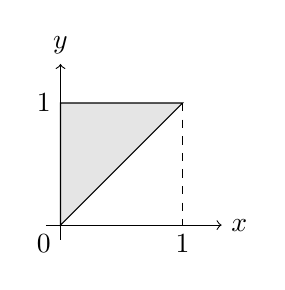
\begin{tikzpicture}[scale=1.55]
\fill[gray!20] (0,0)--(0,1)--(1,1)--cycle;
\draw[->] (-0.12,0)--(1.32,0) node[right] {$x$};
\draw[->] (0,-0.12)--(0,1.32) node[above] {$y$};
\draw (0,0)--(0,1)--(1,1)--cycle;
\draw[dashed] (1,1)--(1,0);
\node[below left] at (0,0) {$0$};
\node[below] at (1,0) {$1$};
\node[left] at (0,1) {$1$};
\end{tikzpicture}
\end{minipage}\hfill
\begin{minipage}[c]{0.70\linewidth}
領域は $0\le x\le y\le 1$ である。高さ $y$ を固定すると、$x$ は $0$ から $y$ まで動く。したがって
$$
\int_0^1\left(\int_0^y e^{y^2}\,dx\right)dy
=\int_0^1 y e^{y^2}\,dy=\frac{e-1}{2}.
$$
\end{minipage}

\ans{5}
$R>1$ とする。広義積分の定義より、
$$
\begin{aligned}
\int_1^\infty\frac{dx}{(x+1)^{3/2}}
&=\lim_{R\to\infty}\int_1^R\frac{dx}{(x+1)^{3/2}}\\
&=\lim_{R\to\infty}\left(\sqrt{2}-\frac{2}{\sqrt{R+1}}\right)=\sqrt{2}.
\end{aligned}
$$

\newpage
\ans{6}
$u=x+y$, $v=x-y$ を $x,y$ について解くと、$T(u,v)=\left((u+v)/2,(u-v)/2\right)$ となる。そのヤコビアンは
$$
J_T=\frac{\partial(x,y)}{\partial(u,v)}
=\begin{vmatrix}1/2&1/2\\1/2&-1/2\end{vmatrix}=-\frac12 .
$$
である。ヤコビアンの絶対値より $dx\,dy=\tfrac12\,du\,dv$ となる。変換後の積分範囲は $0\le u\le 2$, $0\le v\le 3$ であるから、
$$
\iint_D(x+y)(x-y)\,dx\,dy
=\frac12\int_0^2 u\,du\int_0^3 v\,dv=\frac92 .
$$

\ans{7}
底面 $D=\{(x,y):x^2+y^2\le 1\}$ の各点で、立体の高さは $2-x^2-y^2$ である。極座標に変換すると、体積は
$$
\iint_D(2-x^2-y^2)\,dx\,dy
=\int_0^{2\pi}\!\int_0^1(2-r^2)r\,dr\,d\theta
=2\pi\left(1-\frac14\right)=\frac{3\pi}{2}.
$$

\ans{8}
原点からの距離を $r$、$z$ 軸の正の向きから測る角を $\alpha$、方位角を $\theta$ とする。上半球では $0\le r\le 2$, $0\le\alpha\le\pi/2$, $0\le\theta\le 2\pi$ である。密度は $r^2$、体積要素は $r^2\sin\alpha\,dr\,d\alpha\,d\theta$ だから、質量は
$$
\int_0^{2\pi}\!\int_0^{\pi/2}\!\int_0^2
r^4\sin\alpha\,dr\,d\alpha\,d\theta
=2\pi\cdot 1\cdot\frac{32}{5}=\frac{64\pi}{5}.
$$

\ans{9}\par
\noindent\begin{minipage}[c]{0.40\linewidth}
\centering
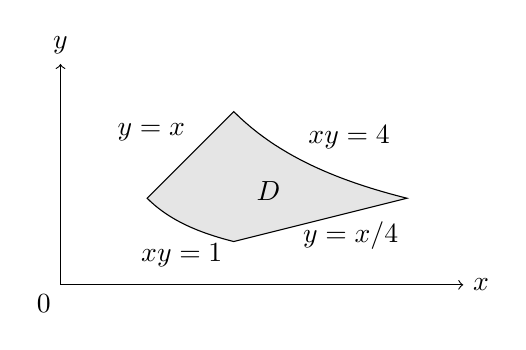
\begin{tikzpicture}[x=1.1cm,y=1.1cm]
\filldraw[fill=gray!20,draw=black]
  plot[domain=1:2,samples=25] (\x,{1/\x})
  -- (4,1) -- plot[domain=4:2,samples=30] (\x,{4/\x})
  -- cycle;
\draw[->] (0,0)--(4.65,0) node[right] {$x$};
\draw[->] (0,0)--(0,2.55) node[above] {$y$};
\node[below left] at (0,0) {$0$};
\node[above left] at (1.55,1.55) {$y=x$};
\node[below] at (1.40,{1/1.40-0.13}) {$xy=1$};
\node[above right] at (2.75,{4/2.75}) {$xy=4$};
\node[below] at (3.35,{3.35/4}) {$y=x/4$};
\node at (2.4,1.08) {$D$};
\end{tikzpicture}
\end{minipage}\hfill
\begin{minipage}[c]{0.57\linewidth}
(1)\enspace $x,y>0$ で条件を書き直すと、$1/x\le y\le 4/x$ かつ $x/4\le y\le x$ となる。これらを同時に満たすのが図の灰色部分である。境界の交点は $(1,1)$、$(2,1/2)$、$(4,1)$、$(2,2)$ である。
\end{minipage}

(2)\enspace $u=xy$, $v=x/y$ とおくと、$x=\sqrt{uv}$, $y=\sqrt{u/v}$ であり、積分範囲は $1\le u\le4$, $1\le v\le4$ となる。ヤコビアンは
$$
\frac{\partial(x,y)}{\partial(u,v)}
=\begin{vmatrix}x/(2u)&x/(2v)\\y/(2u)&-y/(2v)\end{vmatrix}
=-\frac{xy}{2uv}=-\frac{1}{2v}
$$
である。$x^2+y^2=u(v+1/v)$ だから、
$$
I=\int_1^4\!\int_1^4\frac u2(1+v^{-2})\,dv\,du
=\frac{15}{4}\left(3+\frac34\right)=\frac{225}{16}.
$$

\newpage
\ans{10}\par
(1)\enspace 極座標では面積要素が $r\,dr\,d\varphi$ なので、
$$
\begin{aligned}
M&=\int_0^{2\pi}\int_0^R f(r\cos\varphi,r\sin\varphi)\,r\,dr\,d\varphi,\\
H(\theta)&=\int_\theta^{\theta+\pi}\int_0^R f(r\cos\varphi,r\sin\varphi)\,r\,dr\,d\varphi.
\end{aligned}
$$

(2)\enspace $H(\theta)$ と $H(\theta+\pi)$ は、同じ直線で分けた二つの半円に載ったチーズの質量である。共通の境界は面積が $0$ なので、$H(\theta)+H(\theta+\pi)=M$ である。したがって $H(0)-M/2$ と $H(\pi)-M/2$ は互いに符号が反対か、ともに $0$ である。$H$ は連続なので、中間値の定理より $H(\theta)=M/2$ を満たす $\theta\in[0,\pi]$ が存在する。この直線は円の中心を通るため、面積も二等分する。

(3)\enspace 円板の対称性により $x$ と $y$ の項の積分はともに $0$ なので、$M=\rho_0\pi R^2$ である。(1) の式で $r$ について先に積分すると、
$$
\begin{aligned}
H(\theta)
&=\rho_0R^2\int_\theta^{\theta+\pi}
\left(\frac12+\frac{\cos\varphi}{6}+\frac{\sin\varphi}{9}\right)d\varphi\\
&=\frac M2+\frac{\rho_0R^2}{9}\bigl(2\cos\theta-3\sin\theta\bigr).
\end{aligned}
$$
面積を二等分する直線は円の中心を通る。実際、中心からずれた直線では、中心を含む側に半円に加えて正の面積をもつ部分ができる。チーズの質量を二等分する条件は $H(\theta)=M/2$、すなわち $2\cos\theta-3\sin\theta=0$ である。したがって、求める直線の方程式は $2x-3y=0$ である。

\ans{11}
$y=2-3/(x+1)$ と書けるので、$x>-1$ に対応する $y$ の範囲は $y<2$ である。$y(x+1)=2x-1$ を $x$ について解くと、逆関数は $f^{-1}(y)=(y+1)/(2-y)$ となる。定義域は $(-\infty,2)$ である。

\ans{12}
$1/((x+1)(x+2))=1/(x+1)-1/(x+2)$ だから、
$$
\int_0^1\frac{dx}{(x+1)(x+2)}
=\left[\log(x+1)-\log(x+2)\right]_0^1=\log(4/3).
$$

\ans{13}
$x^3y$ は $x$ について奇関数なので、各 $y$ に対する $[-1,1]$ 上の積分は $0$ である。したがって
$$
\iint_D(x^3y+y^2)\,dx\,dy=2\int_0^2 y^2\,dy=\frac{16}{3}.
$$

\newpage
\ans{14}
各小長方形の面積は $1/2$ であり、代表点は $(1,1/2)$、$(1,1)$、$(2,1/2)$、$(2,1)$ である。リーマン和は
$$
\frac12\left(\frac32+2+\frac52+3\right)=\frac92
$$
となる。

\ans{15}
$x^2=2x$ より交点の $x$ 座標は $0$ と $2$ である。その間では $x^2\le2x$ だから、面積は
$$
\int_0^2\int_{x^2}^{2x}1\,dy\,dx
=\int_0^2(2x-x^2)\,dx=\frac43.
$$

\ans{16}
もとの積分領域は $0\le y\le1$、$\sqrt y\le x\le1$ である。これを $0\le x\le1$、$0\le y\le x^2$ と書き直すと、積分順序を交換した式は
$$
\int_0^1\left(\int_0^{x^2}x^2\,dy\right)dx
$$
となる。

\ans{17}
上端を $1-\varepsilon$（$0<\varepsilon<1$）とした積分から、
$$
\int_0^1\frac{dx}{\sqrt{1-x}}
=\lim_{\varepsilon\downarrow0}\int_0^{1-\varepsilon}\frac{dx}{\sqrt{1-x}}
=\lim_{\varepsilon\downarrow0}2(1-\sqrt{\varepsilon})=2.
$$

\ans{18}
$L>1$ とする。被積分関数は非負で、$[1,L]^2$ 上の積分は $\bigl(\int_1^L x^{-2}\,dx\bigr)^2=(1-1/L)^2$ である。$L\to\infty$ の極限を取ると、広義積分の値は $1$ となる。

\ans{19}
$x=u$、$y=uv$ だから、ヤコビアンは $\partial(x,y)/\partial(u,v)=u$ である。範囲は $1\le u\le2$、$1\le v\le3$ となるので、
$$
\iint_D(y/x)\,dx\,dy
=\int_1^2\int_1^3 uv\,dv\,du=\frac32\cdot4=6.
$$

\ans{20}
極座標では $1\le r\le2$、$0\le\theta\le\pi/2$ で、$x^2+y^2=r^2$ である。よって
$$
\iint_D(x^2+y^2)\,dx\,dy
=\int_0^{\pi/2}\int_1^2 r^3\,dr\,d\theta
=\frac{\pi}{2}\cdot\frac{15}{4}=\frac{15\pi}{8}.
$$

\newpage
\ans{21}
$x=u$、$y=2v$ とおくと、領域は単位円板 $u^2+v^2\le1$ となる。ヤコビアンは $2$ なので、面積は
$$
\iint_{u^2+v^2\le1}2\,du\,dv=2\pi
$$
である。

\ans{22}
$0\le x\le2$、$0\le y\le2-x$ の各点で、立体の高さは $2-x-y$ である。よって体積は
$$
\int_0^2\int_0^{2-x}(2-x-y)\,dy\,dx
=\frac12\int_0^2(2-x)^2\,dx=\frac43.
$$

\ans{23}
円柱座標では $0\le r\le2$、$0\le\theta\le2\pi$、$0\le z\le2-r$ である。体積要素は $r\,dz\,dr\,d\theta$ だから、体積は
$$
\int_0^{2\pi}\int_0^2\int_0^{2-r}r\,dz\,dr\,d\theta
=2\pi\int_0^2(2-r)r\,dr=\frac{8\pi}{3}.
$$

\ans{24}
球面座標の動径を $r$、$z$ 軸の正の向きから測る角を $\alpha$、方位角を $\theta$ とすると、範囲は $1\le r\le2$、$0\le\alpha\le\pi$、$0\le\theta\le2\pi$ である。体積は
$$
\int_0^{2\pi}\int_0^\pi\int_1^2 r^2\sin\alpha\,dr\,d\alpha\,d\theta
=2\pi\cdot2\cdot\frac73=\frac{28\pi}{3}.
$$

\ans{25}
円柱座標で密度は $1+r^2$ であり、範囲は $0\le r\le1$、$0\le\theta\le2\pi$、$0\le z\le2$ である。質量は
$$
\int_0^{2\pi}\int_0^1\int_0^2(1+r^2)r\,dz\,dr\,d\theta
=4\pi\left(\frac12+\frac14\right)=3\pi.
$$

\ifPDFTeX
\end{CJK}
\fi
\end{document}
